\documentclass[../root]{subfiles}
\graphicspath{{_images/}{../_images/}}

\begin{document}

    \chapter{Bunching to Maximize Tax Credits: Evidence from Kinks in the U.S. Tax Schedule}

    \begin{shortsummary}
        \begin{itemize}
            \item \authoryear{Mortenson}
            \item \RQ{why does bunching occur at some kinks but not others?}
            \item \answer{Bunching estimation using a panel data of tax returns}
            \item \result{Bunching is particularly responsive at kinks that maximize taxpayer refunds}
        \end{itemize}
    \end{shortsummary}

    \section{Introduction}

    A growing field of public finance: bunching at kink points
    %
    \begin{itemize}
        \item A kink: an income amount for a given taxpayer at which marginal tax rates change discretely, marking the end of one tax bracket and the begging of the next.
    \end{itemize}
    %
    This paper investigates why bunching occurs at some kinks but not others,
    using several major tax acts.
    %
    \begin{itemize}
        \item These acts allow to observe changes in bunching patterns in response to changes in kink locations.
        \item Saez (2010) finds bunching only among self-employed taxpayers and only at the first EITC kinks, not at the second EITC kink or at the largest kink in the statutory schedule.
        \item A potential explanation for this is that some taxpayers may earn or report incomes to maximize refunds, while an alternative explanation is kinks may not be large enough to overcome optimization frictions including the costs of learning about incentives and responding to them.
        \item While Saez (2010) is unable to distinguish them due to sample period, this paper can overcome, expanding sample period: 1960-2014.
    \end{itemize}
    %
    This paper makes four contributions:
    \begin{enumerate}
        \item measures the overall extent of bunching at tax kinks in the U.S.;
        \item shows that many taxpayers gravitate towards the unique point of the tax schedule that maximizes the refund they receive.
        \item shows that bunching at refund-maximizing kinks is partly driven by persistence
        \item documents the emergence of bunching by war earners and shows that this is driven exclusively by income misreporting. 
    \end{enumerate}

    \begin{figure}[t]
        \centering
        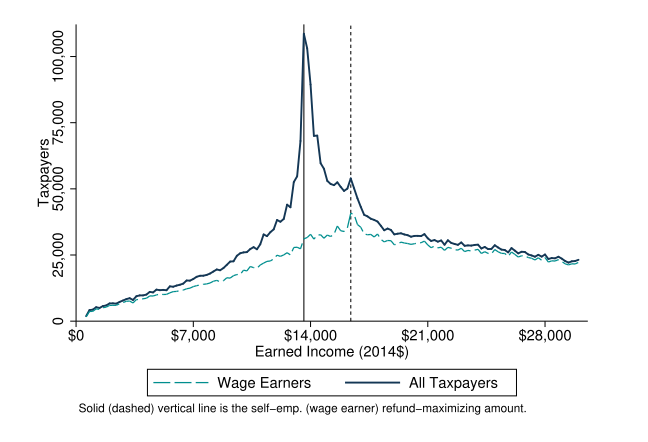
\includegraphics[width = 0.8\linewidth]{0626kato/fig1.PNG}
        \caption{Pooled distribution of taxpayers: Single taxpayers with 2 children in 2014}
        \label{fig1}
    \end{figure}

    Figure \ref{fig1} demonstrates main findings:
    \textit{bunching in the figure is mostly due to the self-employed, 
    but wage earners bunch as well,
    and both groups appear drawn to kinks that maximize refunds.}
    %
    \begin{itemize}
        \item This phenomenon is growing rapidly (0.5 percent of EITC-eligible taxpayers in 1996, but 2.1 percent of EITC-eligible taxpayers in 2014).
        \item Easy learning: tax-filing software is correlated with locating near the refund-maximization kink, which implies that this system gives taxpayers a chance to learn bunching incentives.
        \item Since the most common way of bunching is by reporting self-employment income, we raises the question of whether their bunching reflects distortions of real economic behavior or merely reporting decisions. They cannot definitively answer.
    \end{itemize}

    
    \section{Data and Estimation}

    \subsection{Data}

    Main sample: Panel data of 258 million tax returns that is representative of the tax-filing population in the United States in every year from 1996 to 2014.
    %
    \begin{itemize}
        \item data drawn from the population of federal income tax returns (filed by taxpayers) and information returns (typically filed by third parties, e.g. employer-reported wage income called Form W-2) of individuals in the U.S.
        \item Use information on date of birth and sex at the time of birth from the Social Security Administration's Data Master File.
        \item All data are pre-audit and therefore reflect what taxpayers report when filing, including any errors.
    \end{itemize}
    %
    Combined Sample
    %
    \begin{itemize}
        \item The panel is unbalanced
        \item when we track taxpayers over time, they supplement the Main Sample with an auxiliary dataset that includes all observations of tax units whose secondary filer is a primary filer in at least one year in our Main Sample.
    \end{itemize}

    \subsection{Estimation of Bunching}

    \begin{figure}[t]
        \centering
        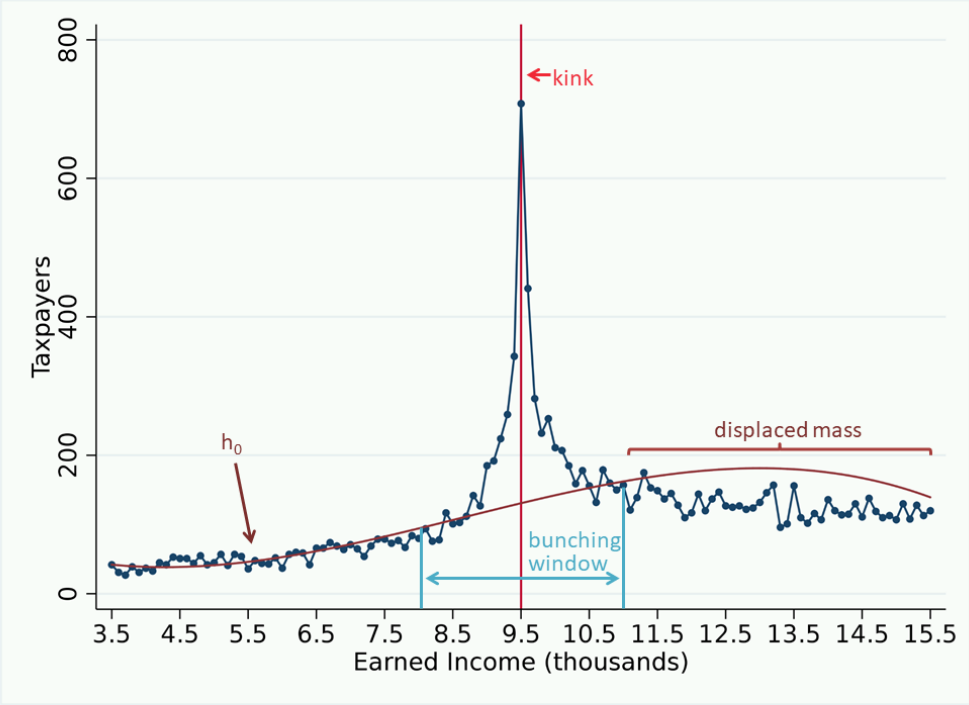
\includegraphics[width = 0.8\linewidth]{0626kato/fig3.PNG}
        \caption{Example of Bunching Estimation}
        \label{}
    \end{figure}
    
    Key issues: How taxpayers would behave in the absence of a kink (counterfactual).
    %
    \begin{itemize}
        \item Specify an alternative (local) tax schedule as well as the (local) distribution of income under the alternative tax schedule.
        \item Let $t_0$ denote the marginal tax rate that applies below a given kink $z^*$, and $t_1$ the rate that applies above it.
    \end{itemize}
    %
    Technique: Chetty et al. (2011) estimates the counterfactual scenario in which $t_0$ applies both above and below $z^*$ with in a certain distance surrounding the kink (the "bunching region").
    %
    \begin{itemize}
        \item Note that this removes the kink within the region of study.
        \item To measure the amount of bunching ($\hat{B}$), compare the actual distribution of income with the predicted counterfactual distribution ($h_0$) of income under tax rate $t_0$.
        \item the counterfactual income distribution is predicted by observed data near kink but not so close as to be affected by bunching behavior (exclude the bins immediately surrounding the kink called "the bunching window").
        \item $h_0$ is estimated by the actual distribution of income between \$1,500 and \$6,000 away from each kink. 
        \item a bunching coefficient $\hat{b}$ is equal to the percentage of taxpayers inside the bunching window who are classified as bunchers. 
        \item standard errors for $\hat{B}$ and $\hat{b}$ are calculated by adding randomly sampled estimated residuals from the original regressions to the predicted values of the original regressions (bootstrap procedure).
    \end{itemize}
    %
    Problem 1: to impose integration constraint where the bunchers are reallocated.
    %
    \begin{itemize}
        \item this constraint reallocates them above the bunching window but within the bunching region (the total number of taxpayers within the bunching region is identical in the actual and counterfactual densities).
        \item In this context, some of mass should be reallocated outside of the bunching region (to the next higher kink), which leads to upper bias of $h_0$.
    \end{itemize}
    %
    Problem 2: to remove the kink (the incentive to bunch) within region of study 
    %
    \begin{itemize}
        \item Suppose that we wish to analyze kink $K$, but kink $L$ lies somewhere inside $K$'s bunching window.
        \item This method may identify bunchers at kink $L$ as responding to kink $K$ (misattribution)
        \item To deal with this, they estimate the total number of bunchers in the usual way. and assign fraction $\Delta t_k/(\Delta t_K + \Delta t_L)$ to the bunchers to $K$, and one minus this fraction to$L$ where $\Delta t_j$ is marginal tax rates change at kink $j$.  
    \end{itemize}


    \section{Results}

    \subsection{Bunching at Refund Maximization?}

    \begin{figure}[t]
        \centering
        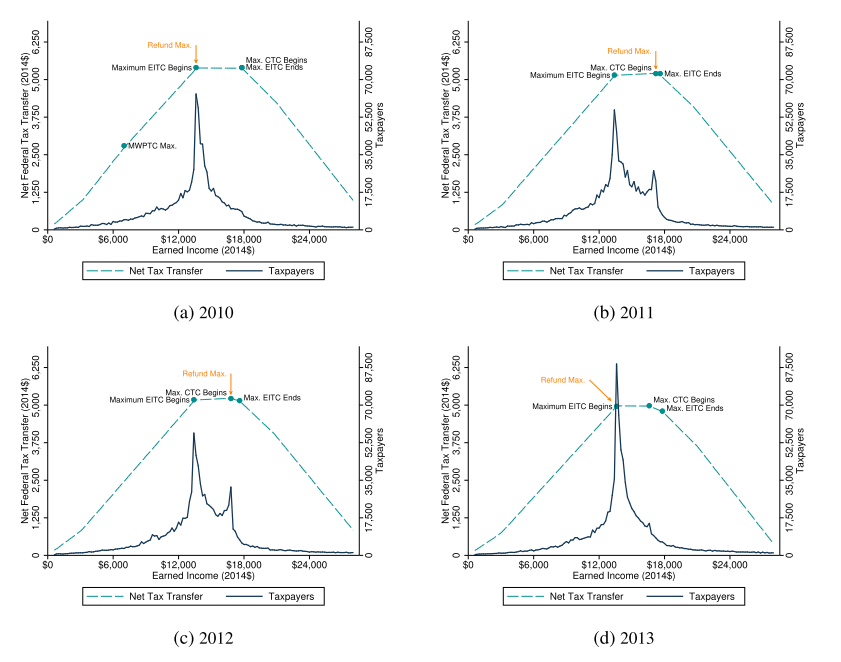
\includegraphics[width = 0.8\linewidth]{0626kato/fig6.PNG}
        \caption{Tracking the refund-maximizing kink: Singles with two children and with self-employment income}
        \label{fig6}
    \end{figure}

    Some taxpayers immediately respond to this minor change in the tax code by shifting to the new refund maximization (Figure \ref{fig6}).
    %
    \begin{itemize}
        \item Relative to 2010, the 2011 income distribution features significantly less bunching at the first EITC kink (the refund-maximizing kink in 2010) and significantly more at the CTC kink (the refund-maximizing kink in 2011).
        \item The refund-maximizing kink for these taxpayers is the first EITC kink for 92 percent in 2010, 24 percent in 2011 and 2012, and 93 percent in 2013, and the CTC kink for 58 percent in 2011 and 2012.
    \end{itemize} 


    \subsection{Distort Real Economic Activity to Maximize Refund? Noncompliance to Maximize Refund?}

    \begin{figure}[t]
        \centering
        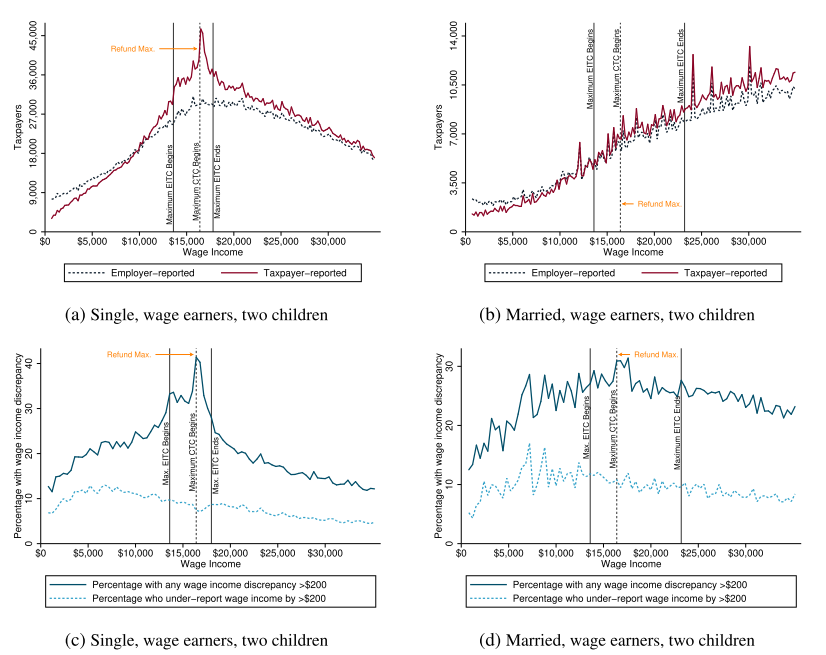
\includegraphics[width = 0.8\linewidth]{0626kato/fig8.PNG}
        \caption{Taxpayer- and employer-reported wage income (2014)}
        \label{fig8}
    \end{figure}
    
    Test for noncomplaince by comparing taxpayer- and employer- reported income
    %
    \begin{itemize}
        \item Due to third-party reporting, wage income has been shown to exhibit significantly less non-compliance than self-employment income. Thus, wage-earner bunching provides prima facie evidence of real labor supply or real labor demand responses. 
        \item However, it remains possible that wage-earners bunching is due to noncomplaince. 
    \end{itemize}
    %
    Result: The excess mass of wage earners near kinks is wholly due to misreported earnings (Figure \ref{fig8}).
    %
    \begin{itemize}
        \item Relative to employer-reported income, taxpayer-reported income features additional mass in the EITC plateau region (between the two solid vertical bars) for the single taxpayers of panel (a). This extra mass exhibits sharp bunching precisely at the CTC kink, which maximized refunds.
        \item There is little excess mass in the EITC plateau region and no bunching in either taxpayer-reported or employer-reported wages for the married taxpayers of panel (b).
        \item Panel (c) and (d) display the percentage of taxpayers in a given income bin who have a discrepancy between their employer- and taxpayer-reported incomes greater than \$200.
        \begin{itemize}
            \item Taxpayers reporting incomes in the bins containing the first EITC kink and the CTC kink are more likely to have a wage-income discrepancy.
            \item Wage income discrepancies are not driven by under-reporting. This means bunching due to wage incomes discrepancies is driven by taxpayers reporting incomes exceeding those their employers report.
        \end{itemize}
    \end{itemize}

    Probit regression to explore the characteristics of correlated with refund maximization
    %
    \begin{itemize}
        \item Motivation: Due to the incomplete nature of third-party reporting of self-employment earnings, an analogous exercises for the self-employed is not possible.
        \item Outcome: an indicator whether the taxpayer is within \$500 of their refund-maximizing kink.
        \item Result: Both wage earners and the self-employed are somewhat more likely to maximize refunds when no W-2 (employer-reported wage income) is present to substantiate wage income.
    \end{itemize}


    \subsection{Dynamics in Refund Maximization}

    \begin{figure}[t]
        \centering
        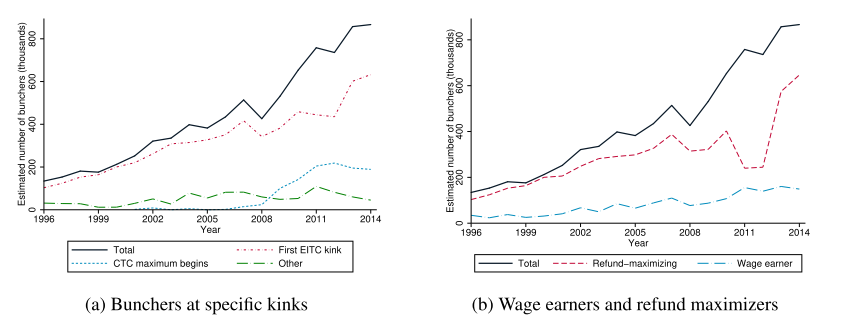
\includegraphics[width = 0.8\linewidth]{0626kato/fig5.PNG}
        \caption{Bunching over time}
        \label{fig5}
    \end{figure}

    The change of the number of bunchers over time (figure \ref{fig5}).
    %
    \begin{itemize}
        \item The number of bunchers at refund-maximizing kinks grew from 103,100 in 1996 to 646,600 in 2014 - a 527 percent increase, but was non-monotonic as panel (b).
        \item During off-trend period, many taxpayers saw their refund-maximizing kink change location and identity. For the majority of taxpayers the refund-maximizing kink was no longer the first EITC kink, where bunching levels generally continued to climb as panel (a) shows.
        \item Panel (b) shows that substantial wage-earner bunching is a relatively recent phenomenon.
    \end{itemize}

    \begin{figure}[t]
        \centering
        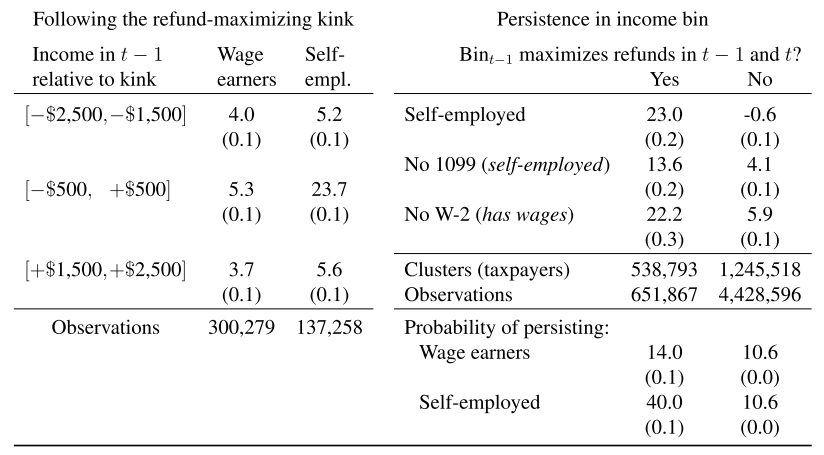
\includegraphics[width = 0.8\linewidth]{0626kato/tab3.PNG}
        \caption{Dynamic responses to refund-maximizing kinks (2005-2014)}
        \label{tab3}
    \end{figure}

    \noindent
    Tracking the refund-maximizing kink when it moves
    (the first three columns on the left of figure \ref{tab3}).
    %
    \begin{itemize}
        \item The probability of reporting income in certain ranges relative to the refund-maximizing kink in year $t$ conditional on year $t-1$ income.
        \item The sample is limited to taxpayers who saw the refund-maximizing kink move by at least \$2,000 (in 2014 dollars) between years $t-1$ and $t$.
        \item Around 24 percent of self-employed taxpayers who were within \$500 of the refund-maximizing kink in year $t-1$ manage to locate near the kink again in year $t$.
        \item Taxpayers may unintentionally track refund-maximizing kinks due to income volatility. $\Rightarrow$ the probabilities of a similar income change either \$2,000 above or below the refund-maximizing kink are between five ans six percent.
        \item Differencing out this income volatility yields an estimate that around 18 and 19 percent of self-employed taxpayers maximizing refunds in a given year will intentionally maximize refunds in the subsequent year, conditional on the refund-maximizing kink substantially shifting locations.
        \begin{itemize}
            \item One to two percent of wage earners who maximize refunds in a given year will intentionally maximize refunds the following year.
        \end{itemize}  
    \end{itemize}
    
    \noindent
    Remaining at the kink when it does not move
    (the columns on the right side of figure \ref{tab3}).
    %
    \begin{itemize}
        \item Away from refund-maximizing kinks, the self-employed are equally likely as wage earners to persist in the same income bin from year to year.
        \item In refund-maximizing bins, the self-employed are 26 percentage points more likely to persist than wage earners (14.0 percent and 40.0 percent).
    \end{itemize}


    \section{Concluding Remarks}

    \begin{quote}
        ..., we have uncovered several new facts about taxpayer bunching in the United States. Most notably, we have shown that bunching is particularly responsive at kinks that maximize taxpayer refunds. For many groups, when the refund-maximizing kink changes location between consecutive years, a large mass of taxpayers appears at the new refund-maximizing kink (\citealp[p.19]{Mortenson}). 
    \end{quote}


    \biblio

\end{document}